%% ============================================================
%% supplementary.tex — Supplementary Materials
%% When Design Decisions Go to the Agent
%% ============================================================

\documentclass[review]{elsarticle}

\usepackage{amsmath,amssymb}
\usepackage{booktabs}
\usepackage{graphicx}
\usepackage[hidelinks]{hyperref}

\begin{document}

\begin{frontmatter}
\title{Supplementary Materials: When Design Decisions Go to the Agent --- A Governance Experiment in a Virtual Battery Factory}
\author[inst1]{Naiming Xie}
\author[inst1]{Yuan Wang}
\author[inst1]{Mingshan Li}
\affiliation[inst1]{organization={College of Economics and Management, Nanjing University of Aeronautics and Astronautics}, city={Nanjing}, country={China}}
\end{frontmatter}

\appendix

\section{Mechanical Re-Adjudication Rules (Control Conditions)}

The re-adjudication of the control conditions applies the protocol's own
definitions mechanically, by recomputing from artifact files. The rules:

\begin{itemize}
\item \textbf{Plating.} A design plates if the minimum of the anode surface
potential time series (vs.\ Li/Li$^+$) during the 4C charge is below
$0$ V. A claim of ``safe margin'' phrased in kinetic overpotential is not a
substitute for the potential series; if no potential series exists in the
artifacts, the criterion is \emph{unadjudicable} and counted as failed.
\item \textbf{5C retention.} Computed as the 5C discharge capacity divided
by the 1C discharge capacity of the same cell ($5C/1C$). A ratio computed
against a $C/3$ reference is a different caliber and is recomputed.
\item \textbf{SEI thickness.} Judged on the contract aging model (Chen2020,
ec-reaction-limited SEI kinetics) with the design's full declared parameters.
A design that reports SEI from a different growth law (e.g., the
solvent-diffusion-limited variant) is recomputed under the contract
model---the SEI model option is a contract-caliber fixture, not a design
lever.
\item \textbf{Thermal runaway / nail penetration.} Judged by the trigger
criterion of the three-side-reaction ODE solver (\texttt{run-tr}):
\texttt{triggered} must be \texttt{False}. A steady-state hotspot
temperature is not a trigger criterion.
\item \textbf{Measurement space.} A design is out-of-space if its chemistry
or model is not reproducible by the protocol's verified parameter sets
(Chen2020, ORegan2022, OKane2022, Prada2013); such designs are documented
separately and excluded from the same-space attainment counts.
\end{itemize}

\section{C1 Re-Adjudication Detail}

Table~\ref{tab:c1supp} restates the main-text table with the exact values
and the failing criterion per task.

\begin{table}[!htbp]
\centering
\caption{Protocol-free agent claims vs.\ contract-caliber re-adjudication.}
\label{tab:c1supp}
\begin{tabular}{p{1.0cm}p{4.2cm}p{3.2cm}p{5.4cm}}
\toprule
Task & Self-reported & Re-adjudicated value & Failing criterion \\
\midrule
T1 & ``safe'' plating margin & min $\eta=-6.9$ mV & $<0$ V $\Rightarrow$ plated \\
T2 & SEI 8.1/15.1 nm ``all verified'' & 818.9 nm @500 cyc (contract model, full design); 4C plating $-360.9$ mV & SEI $\leq 550$ nm @500 cyc; no plating \\
T3 & 5C retention 96.7\% & 84.8\% ($5C/1C$) & retention $\geq 95\%$ \\
T4 & achieved (Li-metal cell) & --- & out-of-space \\
T5 & $|\eta|$ ``3--4$\times$ safe'' & min $\eta=-12.6$ mV & $<0$ V; no series \\
T6 & (no deliverable) & --- & budget exhausted \\
T7 & ``all met'' & hotspot 118.5\,$^\circ$C & no trigger criterion \\
T8 & achieved (Li-metal cell) & --- & out-of-space \\
\bottomrule
\end{tabular}
\end{table}

\begin{figure}[!htbp]
\centering
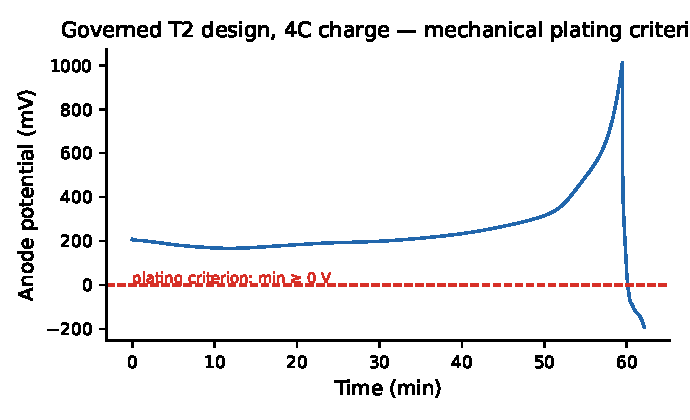
\includegraphics[width=0.8\linewidth]{figs/fig_supp_plating.pdf}
\caption{The mechanical plating criterion as applied: anode potential time
series of the governed T2 design during 4C charge, with the $0$ V line.
A design plates if and only if the minimum crosses this line.}
\label{fig:splating}
\end{figure}

\begin{figure}[!htbp]
\centering
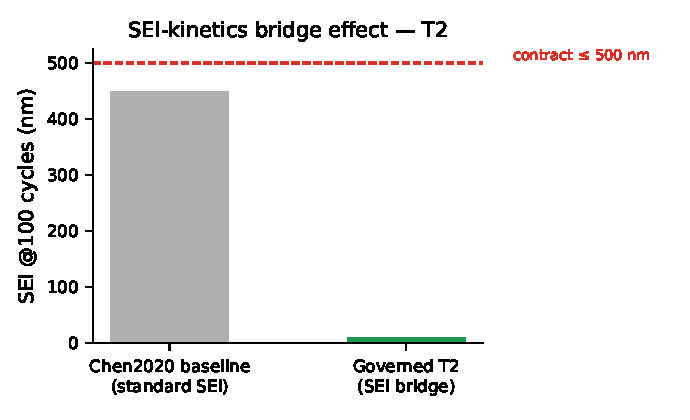
\includegraphics[width=0.8\linewidth]{figs/fig_supp_sei.pdf}
\caption{SEI-kinetics bridge effect on T2: Chen2020 baseline SEI after 100
cycles versus the governed design's bridged value, against the 500 nm
contract line.}
\label{fig:ssei}
\end{figure}

\section{Task--Product Anchoring Table}

The thresholds in the task texts are calibrated from the underlying
parameter sets at the DFN contract caliber (mechanically derived via
\texttt{calc-energy}); the anchoring is a Methods-section record and never
appears in the task text seen by any agent.

\begin{table}[!htbp]
\centering
\caption{Scenario anchoring and threshold calibration sources.}
\label{tab:anchor}
\begin{tabular}{p{1.0cm}p{5.6cm}p{6.6cm}}
\toprule
Task & Anchored scenario & Calibration source \\
\midrule
T1 & LG M50T fast-charge EV (4C + thermal red line) & ORegan2022 contract-caliber baseline 327.18 Wh/kg $\rightarrow$ target 392.61 (+20\%) \\
T2 & Grid storage (cycle + low temperature) & OKane2022 100-cycle SEI baseline 626.8 nm $\rightarrow$ 500 nm limit; Chen2020 low-T retention 99.5\% $\rightarrow$ 90\% limit \\
T3 & Power-tool high-rate & OKane2022 5C/1C $\approx$ 100\% $\rightarrow$ 95\%; power baseline 3814 $\rightarrow$ 4000 W/kg \\
T4 & Extreme-cold equipment & OKane2022 volumetric baseline 854 $\rightarrow$ 880 Wh/L \\
T5 & Flagship extreme verification & Chen2020 contract baseline 400.75 $\rightarrow$ 500.94 Wh/kg \\
T6 & Smartphone (volumetric + temperature red line) & OKane2022 854 $\rightarrow$ 950 Wh/L; NMC811 plateau limit 4.03 V $\rightarrow$ 4.1 V \\
T7 & Hybrid (high-temperature + nail) & 45\,$^\circ$C 100-cycle SEI $\leq 550$ nm; 10 W nail penetration \\
T8 & Long-endurance drone & OKane2022 baseline 405.62 $\rightarrow$ 446.18 Wh/kg; mass $\leq 40$ g \\
\bottomrule
\end{tabular}
\end{table}

\section{Contract Margins of the Governed Runs}

Margins are computed mechanically from the evidence chains of the final
passing evaluations: $\text{margin} = (v - t)/|t|$ for minimum thresholds
and $(t - v)/|t|$ for maximum ones, with $v$ the evidence value and $t$ the
pre-registered threshold. Boolean criteria (plating, thermal-runaway
trigger) pass exactly and carry no margin.

\begin{table}[!htbp]
\centering
\caption{Per-criterion margins of the eight governed runs (pro model).
The left column lists the criterion each task cleared last (binding
margin); the right column lists the wide-margin criteria.}
\label{tab:margins}
\begin{tabular}{p{1.0cm}p{5.4cm}p{3.4cm}p{4.2cm}}
\toprule
Task & Binding criterion (value vs threshold) & Margin & Wide margins \\
\midrule
T1 & $T_{\max}$ 325.65 vs 333.15 K & $+2.2\%$ & ED 553.98 vs 392.61 ($+41.1\%$) \\
T2 & low-T retention 99.57 vs 90\% & $+10.6\%$ & ED 465.62 vs 327.18 ($+42.3\%$); SEI 9.1 vs 500 nm ($+98.2\%$) \\
T3 & $T_{\max}$ 329.77 vs 333.15 K & $+1.0\%$ & power 32\,630 vs 4000 W/kg ($+716\%$); 5C retention 97.53 vs 95\% ($+2.7\%$) \\
T4 & low-T retention 99.27 vs 95\% & $+4.5\%$ & Wh/L 925.8 vs 880 ($+5.2\%$); ED 471.55 vs 327.18 ($+44.1\%$) \\
T5 & $T_{\max}$ 328.13 vs 333.15 K & $+1.5\%$ & ED 641.83 vs 500.94 ($+28.1\%$) \\
T6 & plateau 4.1145 vs 4.1 V & $+0.4\%$ & Wh/L 1135.8 vs 950 ($+19.6\%$); $T_{\max}$ 321.42 vs 323.15 K ($+0.5\%$) \\
T7 & SEI 465.5 vs 550 nm & $+15.4\%$ & ED 483.25 vs 327.18 ($+47.7\%$) \\
T8 & mass 39.8 vs 40 g & $+0.5\%$ & ED 634.32 vs 446.18 ($+42.2\%$); 5C retention 98.77 vs 90\% ($+9.7\%$) \\
\bottomrule
\end{tabular}
\end{table}

BO seed robustness. The Bayesian baseline is deterministic in its seed, and
a three-seed replication (1234, 5678, 9012) leaves the attained-task set
unchanged. Attaining-trial counts per task and seed (out of 50 evaluations):

\begin{table}[!htbp]
\centering
\caption{BO contract-attaining trials per task across three seeds
(mechanical criteria as in the main text; the attained-task set is
$\{T1, T4, T8\}$ in every seed).}
\label{tab:boseeds}
\begin{tabular}{lccc}
\toprule
Task & seed 1234 & seed 5678 & seed 9012 \\
\midrule
T1 & 25 & 28 & 21 \\
T2 & 0 & 0 & 0 \\
T3 & 0 & 0 & 0 \\
T4 & 34 & 33 & 32 \\
T5 & 0 & 0 & 0 \\
T6 & 0 & 0 & 0 \\
T7 & 0 & 0 & 0 \\
T8 & 10 & 5 & 1 \\
\bottomrule
\end{tabular}
\end{table}

The SEI criteria are adjudicated on the contract aging model (Chen2020,
ec-reaction-limited), in which the electrode-modification bridge scales the
SEI kinetic rate constant $k_{\mathrm{SEI}}$ (standard $10^{-12}$ m/s).
The governed runs used this lever as follows. T2 shipped $k_{\mathrm{SEI}} =
10^{-16}$ m/s ($10^{-4}\times$), declared in the audit as an estimate
beyond the bare-ALD literature magnitude under a dual-mechanism coating
claim (ALD plus fluorinated-additive inner SEI); the same design at
$10^{-14}$ m/s ($10^{-2}\times$) meets the identical contract, with the
500-cycle SEI at 500.4 nm against the 550 nm limit---a $9\%$ margin---so
the T2 SEI criteria do not hinge on the extreme setting. T6's SEI work uses
a $0.5\times$ solvent-diffusivity and concentration cut, derived from the
model's own diffusion-limited rate law, and no T6 verdict depends on SEI.
T7 uses no kinetic override; its 465.5 nm SEI follows from the design
itself.

\section{Real-Data Alignment: Source and License}

The real-data anchor uses the LG M50 battery degradation dataset
(Imperial College London), Zenodo record 10.5281/zenodo.10637534, licensed
under CC BY 4.0, accompanying the paper by Kirkaldy et al.\
(10.1016/j.jpowsour.2024.234185). The comparison is against Experiment 5
(standard cycle aging), Cell A, RPT0 (beginning of life), $0.1$C discharge.

\section{Replication Runs (N=3, All Eight Tasks)}

Three seeds of every task under the governed protocol, deepseek-v4-pro,
same budget as the main matrix.

\begin{table}[!htbp]
\centering
\caption{Threefold replication of all eight tasks.}
\label{tab:replication}
\begin{tabular}{llll}
\toprule
Task & r1 & r2 & r3 \\
\midrule
T1 (structural) & $\checkmark$ 553.98 Wh/kg & $\checkmark$ 583.2 Wh/kg & $\checkmark$ \\
T2 (durability) & $\checkmark$ 465.62 Wh/kg & $\checkmark$ & $\checkmark$ \\
T3 (rate) & $\checkmark$ & $\checkmark$ & $\checkmark$ \\
T4 (cold) & $\checkmark$ 471.55 Wh/kg & $\checkmark$ & $\checkmark$ \\
T5 (flagship) & $\checkmark$ & $\checkmark$ & $\checkmark$ \\
T6 (material) & $\checkmark$ 1135.8 Wh/L & $\checkmark$ & $\checkmark$ \\
T7 (hybrid) & $\checkmark$ & $\checkmark$ & $\checkmark$ \\
T8 (drone) & $\checkmark$ & $\checkmark$ & $\checkmark$ \\
\bottomrule
\end{tabular}
\end{table}

All twenty-four runs achieve their contracts under the mechanical
adjudicator, with complete evidence coverage of every pre-registered
criterion in every run. On T6, all three seeds independently reach the same
material-bottleneck diagnosis and solution---the LNMO system switch---through
three different designs. Contract attainment and the bottleneck diagnosis
are reproducible across seeds; the designs themselves differ.

\section{Positioning vs.\ Battery-Sim-Agent}

Battery-Sim-Agent \cite{chen2026battery} is the closest published system;
Table~\ref{tab:bsa} positions the two papers side by side.

\begin{table}[!htbp]
\centering
\caption{Positioning against Battery-Sim-Agent (KDD 2026).}
\label{tab:bsa}
\begin{tabular}{lll}
\toprule
 & Battery-Sim-Agent & This paper \\
\midrule
Task & inverse parameter estimation (200 synthetic calibration cases) & forward cell design (8 scenario contracts) \\
Objective & curve-matching error & multi-criterion contract attainment \\
Baselines & BO (Ax, seed 1234), CMA-ES, defaults & BO (Ax, seed 1234, same config), protocol-free agent \\
Adjudication & agent-reported error & code-mechanical verdicts + evidence chain \\
Headline & 67--95\% error reduction vs.\ BO & 8/8 vs.\ 3/8 (BO) vs.\ 0/8 in-space (C1) \\
Honesty calibration & low-headroom: BO can tie or win & same low-headroom pattern, plus a yardstick-failure axis BO cannot exhibit \\
\bottomrule
\end{tabular}
\end{table}

\section{Reproducibility Statement}

All simulation protocols, the adjudication layer, and the audit-chain
verifier are distributed with the tool library and pinned by an automated
regression suite. The full code base---protocol, tool library, experiment
harnesses (including the cross-harness legs)---is open source at
\url{https://github.com/wangyuanxty/BatteryDesignAgent}. The audit ledgers (\texttt{log.jsonl}) of every run are
the primary data source of the paper; every table value can be re-derived
mechanically from the ledgers and the tool outputs they reference. LLM runs
are not seed-reproducible; the protocol's verdicts are.

\end{document}
